

% Gradient Info
  
\tikzset {_2xhcrefu0/.code = {\pgfsetadditionalshadetransform{ \pgftransformshift{\pgfpoint{-7.5 bp } { 0 bp }  }  \pgftransformrotate{-225 }  \pgftransformscale{2 }  }}}
\pgfdeclarehorizontalshading{_spn6ydpdw}{150bp}{rgb(0bp)=(0.03,0.22,0.4);
rgb(37.5bp)=(0.03,0.22,0.4);
rgb(62.5bp)=(0,0.29,0.51);
rgb(100bp)=(0,0.29,0.51)}

% Gradient Info
  
\tikzset {_kw0p3luhv/.code = {\pgfsetadditionalshadetransform{ \pgftransformshift{\pgfpoint{-7.5 bp } { 0 bp }  }  \pgftransformrotate{-225 }  \pgftransformscale{2 }  }}}
\pgfdeclarehorizontalshading{_zquv02ocj}{150bp}{rgb(0bp)=(0.03,0.22,0.4);
rgb(37.5bp)=(0.03,0.22,0.4);
rgb(62.5bp)=(0,0.29,0.51);
rgb(100bp)=(0,0.29,0.51)}

% Gradient Info
  
\tikzset {_5nlio4lhy/.code = {\pgfsetadditionalshadetransform{ \pgftransformshift{\pgfpoint{-7.5 bp } { 0 bp }  }  \pgftransformrotate{-225 }  \pgftransformscale{2 }  }}}
\pgfdeclarehorizontalshading{_0px9iulda}{150bp}{rgb(0bp)=(0.03,0.22,0.4);
rgb(37.5bp)=(0.03,0.22,0.4);
rgb(62.5bp)=(0,0.29,0.51);
rgb(100bp)=(0,0.29,0.51)}

% Gradient Info
  
\tikzset {_i9m56ow0g/.code = {\pgfsetadditionalshadetransform{ \pgftransformshift{\pgfpoint{-7.5 bp } { 0 bp }  }  \pgftransformrotate{-225 }  \pgftransformscale{2 }  }}}
\pgfdeclarehorizontalshading{_cp2s0duqo}{150bp}{rgb(0bp)=(0.03,0.22,0.4);
rgb(37.5bp)=(0.03,0.22,0.4);
rgb(62.5bp)=(0,0.29,0.51);
rgb(100bp)=(0,0.29,0.51)}

% Gradient Info
  
\tikzset {_i0ciopkoo/.code = {\pgfsetadditionalshadetransform{ \pgftransformshift{\pgfpoint{-7.5 bp } { 0 bp }  }  \pgftransformrotate{-225 }  \pgftransformscale{2 }  }}}
\pgfdeclarehorizontalshading{_pfe2kjcao}{150bp}{rgb(0bp)=(0.03,0.22,0.4);
rgb(37.5bp)=(0.03,0.22,0.4);
rgb(62.5bp)=(0,0.29,0.51);
rgb(100bp)=(0,0.29,0.51)}

% Gradient Info
  
\tikzset {_4zjqptm1s/.code = {\pgfsetadditionalshadetransform{ \pgftransformshift{\pgfpoint{-7.5 bp } { 0 bp }  }  \pgftransformrotate{-225 }  \pgftransformscale{2 }  }}}
\pgfdeclarehorizontalshading{_2wsugf3gc}{150bp}{rgb(0bp)=(0.03,0.22,0.4);
rgb(37.5bp)=(0.03,0.22,0.4);
rgb(62.5bp)=(0,0.29,0.51);
rgb(100bp)=(0,0.29,0.51)}
\tikzset{every picture/.style={line width=0.75pt}} %set default line width to 0.75pt        

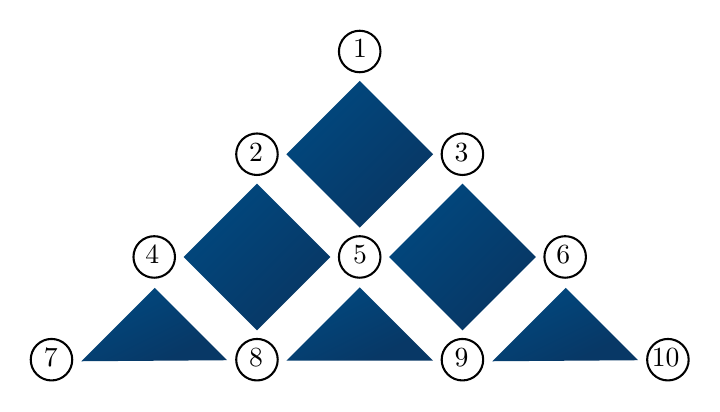
\begin{tikzpicture}[x=0.75pt,y=0.75pt,yscale=-1,xscale=1]
%uncomment if require: \path (0,184); %set diagram left start at 0, and has height of 184

%Shape: Square [id:dp4646069098280107] 
\draw  [draw opacity=0][shading=_spn6ydpdw,_2xhcrefu0] (166.72,29.33) -- (202.08,64.68) -- (166.72,100.04) -- (131.36,64.68) -- cycle ;
%Shape: Circle [id:dp1768374451497594] 
\draw   (159.65,8.11) .. controls (163.55,4.21) and (169.89,4.21) .. (173.79,8.11) .. controls (177.7,12.02) and (177.7,18.35) .. (173.79,22.26) .. controls (169.89,26.16) and (163.55,26.16) .. (159.65,22.26) .. controls (155.74,18.35) and (155.74,12.02) .. (159.65,8.11) -- cycle ;
%Shape: Circle [id:dp9515478681131959] 
\draw   (209.15,57.61) .. controls (213.05,53.71) and (219.38,53.71) .. (223.29,57.61) .. controls (227.19,61.52) and (227.19,67.85) .. (223.29,71.75) .. controls (219.38,75.66) and (213.05,75.66) .. (209.15,71.75) .. controls (205.24,67.85) and (205.24,61.52) .. (209.15,57.61) -- cycle ;
%Shape: Circle [id:dp7756495234805515] 
\draw   (258.64,107.11) .. controls (262.55,103.2) and (268.88,103.2) .. (272.79,107.11) .. controls (276.69,111.01) and (276.69,117.35) .. (272.79,121.25) .. controls (268.88,125.16) and (262.55,125.16) .. (258.64,121.25) .. controls (254.74,117.35) and (254.74,111.01) .. (258.64,107.11) -- cycle ;
%Shape: Circle [id:dp2733517995597814] 
\draw   (110.15,57.61) .. controls (114.06,53.71) and (120.39,53.71) .. (124.29,57.61) .. controls (128.2,61.52) and (128.2,67.85) .. (124.29,71.75) .. controls (120.39,75.66) and (114.06,75.66) .. (110.15,71.75) .. controls (106.25,67.85) and (106.25,61.52) .. (110.15,57.61) -- cycle ;
%Shape: Circle [id:dp7014226103914162] 
\draw   (159.65,107.11) .. controls (163.55,103.2) and (169.89,103.2) .. (173.79,107.11) .. controls (177.7,111.01) and (177.7,117.35) .. (173.79,121.25) .. controls (169.89,125.16) and (163.55,125.16) .. (159.65,121.25) .. controls (155.74,117.35) and (155.74,111.01) .. (159.65,107.11) -- cycle ;
%Shape: Circle [id:dp07847046561305948] 
\draw   (60.65,107.11) .. controls (64.56,103.2) and (70.89,103.2) .. (74.8,107.11) .. controls (78.7,111.01) and (78.7,117.35) .. (74.8,121.25) .. controls (70.89,125.16) and (64.56,125.16) .. (60.65,121.25) .. controls (56.75,117.35) and (56.75,111.01) .. (60.65,107.11) -- cycle ;
%Shape: Right Triangle [id:dp18543834280062976] 
\draw  [draw opacity=0][shading=_zquv02ocj,_kw0p3luhv] (202.08,164.18) -- (131.36,164.18) -- (166.72,128.82) -- cycle ;
%Shape: Right Triangle [id:dp019748006978987376] 
\draw  [draw opacity=0][shading=_0px9iulda,_5nlio4lhy] (300.82,163.93) -- (230.61,164.43) -- (265.97,129.07) -- cycle ;
%Shape: Circle [id:dp3946162772039473] 
\draw   (209.15,156.61) .. controls (213.05,152.7) and (219.38,152.7) .. (223.29,156.61) .. controls (227.19,160.51) and (227.19,166.84) .. (223.29,170.75) .. controls (219.38,174.65) and (213.05,174.65) .. (209.15,170.75) .. controls (205.24,166.84) and (205.24,160.51) .. (209.15,156.61) -- cycle ;
%Shape: Circle [id:dp6620738247447955] 
\draw   (110.15,156.61) .. controls (114.06,152.7) and (120.39,152.7) .. (124.29,156.61) .. controls (128.2,160.51) and (128.2,166.84) .. (124.29,170.75) .. controls (120.39,174.65) and (114.06,174.65) .. (110.15,170.75) .. controls (106.25,166.84) and (106.25,160.51) .. (110.15,156.61) -- cycle ;
%Shape: Circle [id:dp027305429094700795] 
\draw   (11.16,156.61) .. controls (15.06,152.7) and (21.39,152.7) .. (25.3,156.61) .. controls (29.2,160.51) and (29.2,166.84) .. (25.3,170.75) .. controls (21.39,174.65) and (15.06,174.65) .. (11.16,170.75) .. controls (7.25,166.84) and (7.25,160.51) .. (11.16,156.61) -- cycle ;
%Shape: Circle [id:dp5838580222665838] 
\draw   (308.14,156.61) .. controls (312.05,152.7) and (318.38,152.7) .. (322.28,156.61) .. controls (326.19,160.51) and (326.19,166.84) .. (322.28,170.75) .. controls (318.38,174.65) and (312.05,174.65) .. (308.14,170.75) .. controls (304.24,166.84) and (304.24,160.51) .. (308.14,156.61) -- cycle ;
%Shape: Right Triangle [id:dp051990486144260606] 
\draw  [draw opacity=0][shading=_cp2s0duqo,_i9m56ow0g] (102.83,163.93) -- (32.62,164.43) -- (67.98,129.07) -- cycle ;
%Shape: Square [id:dp556944438890764] 
\draw  [draw opacity=0][shading=_pfe2kjcao,_i0ciopkoo] (216.22,78.82) -- (251.57,114.18) -- (216.22,149.53) -- (180.86,114.18) -- cycle ;
%Shape: Square [id:dp31466343787367357] 
\draw  [draw opacity=0][shading=_2wsugf3gc,_4zjqptm1s] (117.22,78.82) -- (152.58,114.18) -- (117.22,149.53) -- (81.87,114.18) -- cycle ;

% Text Node
\draw (162,8) node [anchor=north west][inner sep=0.75pt]   [align=left] {1};
% Text Node
\draw (112,58) node [anchor=north west][inner sep=0.75pt]   [align=left] {2};
% Text Node
\draw (211,58) node [anchor=north west][inner sep=0.75pt]   [align=left] {3};
% Text Node
\draw (62,107) node [anchor=north west][inner sep=0.75pt]   [align=left] {4};
% Text Node
\draw (162,107) node [anchor=north west][inner sep=0.75pt]   [align=left] {5};
% Text Node
\draw (260,107) node [anchor=north west][inner sep=0.75pt]   [align=left] {6};
% Text Node
\draw (13,157) node [anchor=north west][inner sep=0.75pt]   [align=left] {7};
% Text Node
\draw (112,157) node [anchor=north west][inner sep=0.75pt]   [align=left] {8};
% Text Node
\draw (211,157) node [anchor=north west][inner sep=0.75pt]   [align=left] {9};
% Text Node
\draw (306,157) node [anchor=north west][inner sep=0.75pt]   [align=left] {10};


\end{tikzpicture}
